\documentclass[10pt]{beamer}

\usepackage[T2A]{fontenc}
\usepackage[utf8]{inputenc}
\usepackage[russian,english]{babel}
\usepackage{subfig}
\usepackage[noend]{algorithm,algpseudocode}
\usepackage{amsmath}

\usepackage{booktabs}
\usepackage[scale=2]{ccicons}

\usepackage{pgfplots}
\usepgfplotslibrary{dateplot}

\usepackage{xspace}
\newcommand{\TODO}[1]{\textbf{\textcolor{red}{TODO: #1}}}


\algblockdefx{MRepeat}{EndRepeat}{\textbf{repeat}}{}
\algnotext{EndRepeat}

\algrenewcommand\alglinenumber[1]{\footnotesize #1}
\DeclareMathOperator{\rank}{rank}
\DeclareMathOperator{\sign}{sign}

\newcounter{mycounter}

\newcommand{\myparagraph}{\stepcounter{mycounter}\paragraph{\arabic{mycounter}}}
\usepackage{tikz}
\usetikzlibrary{arrows,positioning} 
\tikzset{
    mynode/.style={rectangle,rounded corners,draw=black, top color=white,very thick, inner sep=1em, text centered},
    mycircle/.style={circle,draw=black, top color=white,very thick, text centered},
    pil/.style={ ->, thick, shorten <=2pt, shorten >=2pt,}
}  

\title{Лекция 7}
\subtitle{Выбор моделей}

\begin{document}

\section{Разбор летучки}

\maketitle

\begin{frame}{Задача выбора метода обучения}
  $X$ - множество объектов \\
	$Y$ - множество классов \\
	Обучающая выборка: ${X^l = (x_i, y_i)_{i=1}^l}$ \\ 
	Целевая функция: $f: X \rightarrow Y$\\
	\bigbreak
	Набор моделей алгоритмов $A_t: X \rightarrow Y$, $t \in T$ \\
	Методы обучения $\mu: (X \times Y)^l \rightarrow A_t$, $t \in T$ \\
	\bigbreak
	\alert{Задача}: Найти алгоритм $a \in A_t$  с наилучшей обобщающей способностью
\end{frame}

\begin{frame}{Модель}
  \begin{tikzpicture}[node distance=1cm, scale=0.8, transform shape]
    \node[mynode, text width=5cm] (target) 
      {Неизвестная целевая функция\\
      \textcolor{blue}{$f: X \rightarrow Y$}};
    \node[mynode, text width=3.5cm, below=1cm of target] (training) 
      {Обучающая выборка\\
      \textcolor{blue}{${X^l = (x_i, y_i)_{i=1}^l}$}}
          edge[pil, <-] (target.south);
    \node[below=1cm of training] (dummy) {}; 
    \onslide<2, 3>{    
      \node[mycircle,text width=1.5cm, below=1cm, right=2cm of dummy] (learning) 
        {Метод обучения\\
        \textcolor{blue}{$\mu_t$}}
        edge[pil, <-, bend left=15] (training.south);  
      }
    \onslide<3>{   
      \node[mynode, text width=3cm, below=1cm of dummy] (hypothesis) 
        {Набор моделей\\
        \textcolor{blue}{$A_t$}}
        edge[pil, bend left=15] (learning.west);  
        }
    \node[mynode, text width=3.5cm, right=1cm of learning] (final) 
      {Финальный алгоритм\\
      \textcolor{blue}{$a \in A_t$}}
      edge[pil, <-] (learning.east);    
  \end{tikzpicture}
\end{frame}

\begin{frame}{Модель}
  \begin{tikzpicture}[node distance=1cm, scale=0.8, transform shape]
    \node[mynode, text width=5cm] (target) 
      {Неизвестная целевая функция\\
      \textcolor{blue}{$f: X \rightarrow Y$}};
    \node[mynode, text width=3.5cm, below=1cm of target] (training) 
      {Обучающая выборка\\
      \textcolor{blue}{${X^l = (x_i, y_i)_{i=1}^l}$}}
          edge[pil, <-] (target.south);
    \node[below=1cm of training] (dummy) {}; 
    \node[mycircle, orange, text width=1.5cm, below=1cm, right=2cm of dummy] (learning) 
      {Метод обучения\\
      \textcolor{blue}{$\mu_t$}}
      edge[pil, <-, bend left=15] (training.south);  
    \node[mynode, orange, text width=3cm, below=1cm of dummy] (hypothesis) 
      {Набор моделей\\
      \textcolor{blue}{$A_t$}}
      edge[pil, bend left=15] (learning.west);  
    \node[mynode, text width=3.5cm, right=1cm of learning] (final) 
      {Финальный алгоритм\\
      \textcolor{blue}{$a \in A_t$}}
      edge[pil, <-] (learning.east);    
  \end{tikzpicture}
\end{frame}

\section{Пример}

\begin{frame}{Перцептрон}
  Набор моделей:\\
  $a(\mathbf{x}) = \sign(\sum\limits_{j=1}^n {\only<2,3>{\color{orange}}w_j} x^j - {\only<2,3>{\color{orange}}w_0})$\\
  \bigbreak
  \pause
  \pause
  Метод обучения:\\
  \begin{algorithmic}[1]
    \Function{perceptron}{$X^l$}
      \State Инициализировать ${w_0, \dots, w_n}$
      \MRepeat [пока $\mathbf{w}$ изменяются] 
         \For {$i = 1, \dots, l$}
           \If {$a(x_i) \neq y_i$}
             \State $\mathbf{w} = \mathbf{w} + y_i \mathbf{x_i}$
           \EndIf  
         \EndFor
       \EndRepeat
     \EndFunction
    \end{algorithmic}
\end{frame}

\begin{frame}{Задача}  
  \centering
  Научиться оценивать метод обучения и обобщающую способность алгоритма
\end{frame}

{\foot{loss function}
\begin{frame}{Функция потерь}
  Функция потерь $\mathcal{L}(a, x_i) $ -- характеризует величину ошибки алгоритма $a$ на объекте $x_i$.\\
  \bigbreak
  Если $\mathcal{L} (a, x_i) = 0$, то ответ $a(x_i)$ называется корректным.
\end{frame}
}

{\foot{loss function}
\begin{frame}\frametitle{Примеры $\mathcal{L}$}
	\begin{figure}[htbp]
	  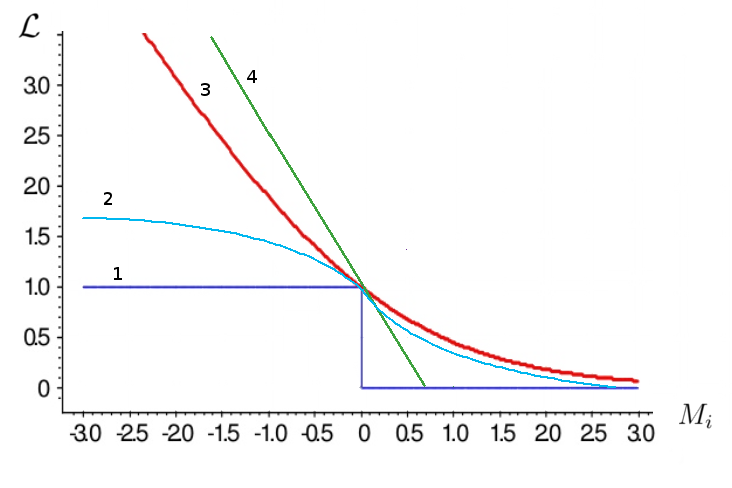
\includegraphics[height=160pt, keepaspectratio = true]{images/l}
	\end{figure}
\end{frame}
}

{\foot{функционал средних потерь, Empirical Risk}
\begin{frame}{Функционал качества}
  Функционал качества алгоритма $a$ на выборке $X^l$:\\
  $$Q(a, X^l) = \frac{1}{l} \sum\limits_{i=1}^l \mathcal{L}(a, x_i)$$\\
  Минимизация эмпирического риска:\\
  $$\arg\min\limits_{A_t} Q(a, X^l)$$
\end{frame}
}

\begin{frame}{Внутренний функционал}  
  $$Q_{\mu}(X^l) = Q(\mu(X^l), X^l)$$\\
  \bigbreak
  Этот функционал оценивает качество обучения на выборке $X^l$\\
  \bigbreak
  \pause
  Какая с этим может быть проблема?
\end{frame}

%\begin{frame}{Простая аналогия}
%  \centering
%  С какой вероятностью монета, подброшенная 10 раз, выпадет одной и той же стороной все 10 раз?
%  \pause
%  \bigbreak
%  \textcolor{blue}{$0.001$}
%\end{frame}
%
%\begin{frame}{Простая аналогия}
%  \centering
%  С какой вероятностью одна из 1000 монет, каждая из которых подброшена 10 раз, выпадет одной и той же стороной все 10 раз?
%  \pause
%  \bigbreak
%  \textcolor{blue}{$0.63$}
%\end{frame}

\begin{frame}{Сложность модели}  
  \centering
  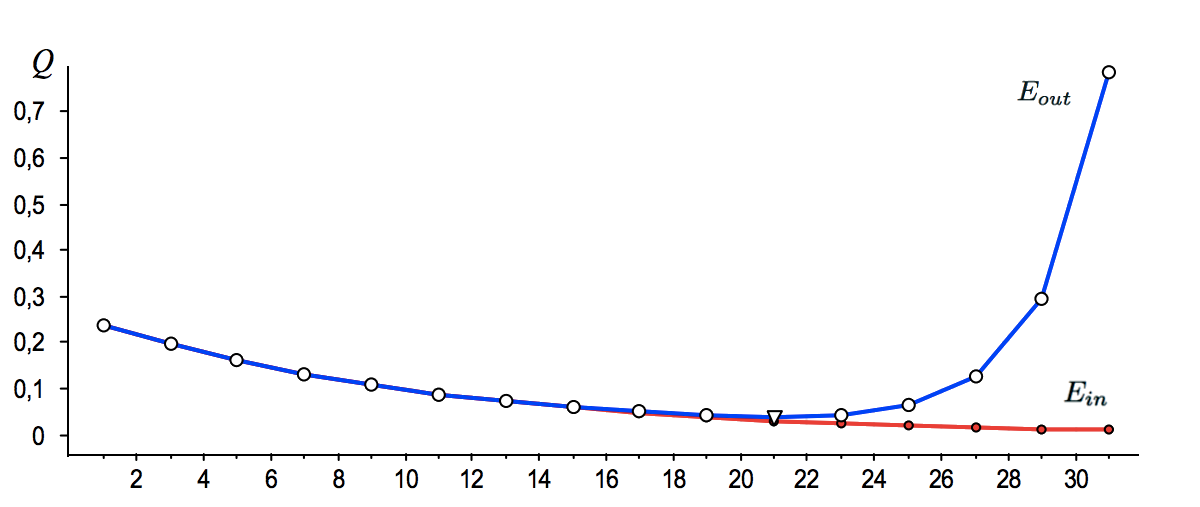
\includegraphics[width=\textwidth]{images/learning_curve}
\end{frame}

\section{Почему случается переобучение?}

%\begin{frame}\frametitle{Проблема переобучения}
%	$a(\mathbf{x}, \mathbf{w}) = sign(\langle \mathbf{w}, \mathbf{x}\rangle)$\\
%	\bigbreak
%	\pause
%	Линейная зависимость признаков:\\
%	$\forall \mathbf{x} \exists \mathbf{u}: \langle \mathbf{u}, \mathbf{x}\rangle = 0$\\
%	$\Rightarrow \forall \gamma: a'(\mathbf{x}, \mathbf{w}) = sign(\langle \mathbf{w} + \gamma \mathbf{u}, \mathbf{x}\rangle)$\\
%	\bigbreak
%	\pause
%	Алгоритм $a'$ работает точно также как исходный $a$.\\
%	А значит мы можем получить любое решение из семейства $\mathbf{w} + \gamma \mathbf{u}$
%\end{frame}

\begin{frame}\frametitle{Проблема переобучения}
	\begin{itemize}
		\item[--] Слишком мало объектов
		\item[--] Слишком много признаков
		\item[--] Линейная зависимость признаков
	\end{itemize}
\end{frame}

\begin{frame}{Внешний функционал}  
  $$E_{in} = Q_{\mu}(X^l) = Q(\mu(X^l), X^l)$$\\
  \bigbreak
  Внешний функционал по отложенной выборке:\\
  $$E_{out} = Q_{\mu}(X^t, X^k) = Q(\mu(X^t), X^k)$$\\
  \bigbreak
  \onslide<2>{
    Какой здесь недостаток?\\
  }
  \onslide<3>{
    Сильная зависимость от разбиения $X^l = X^t \sqcup X^k$
  }
\end{frame}

{\foot{Полный скользящий контроль, cross-validation}
\begin{frame}{Кроссвалидация}  
  \alert{Идея}: Усреднить по всем $C_l^t$ выборкам $X^l = X^t \sqcup X^k$\\
  $$CCV(\mu, X^l) = \frac{1}{C_l^t} \sum\limits_{X^t} Q_{\mu}(X^t, X^k)$$\\
  \bigbreak
  \pause
  Во что превратится оценка при $k=1$?
\end{frame}
}

\begin{frame}{Недостатки}  
  \begin{enumerate}
    \item[--] Оценка вычислительно слишком сложна
    \item[--] Не учитывает дисперсию $X^k$
  \end{enumerate}
\end{frame}

\begin{frame}{k-fold кроссвалидация}  
  \alert{Идея}: Возьмём случайное разбиение $X^l = X_1 \sqcup \dots \sqcup X_k$ на $k$ блоков равной длины.\\
  $$CV_k(\mu, X^l) = \frac{1}{k} \sum\limits_{i=1}^{k} Q_{\mu}(X^l \setminus X_i, X_i)$$\\
  \bigbreak
  \pause
  Недостатки:  
  \begin{enumerate}
    \item[--] Оценка зависит от разбиения на блоки
    \item[--] Каждый объект только один раз участвует в контроле    
  \end{enumerate}
\end{frame}

{\foot{Repeated k-fold cross validation}
\begin{frame}{Повторяющийся k-fold CV}  
  \alert{Идея}: Выборка разбивается $t$ раз случайным образом на $k$ блоков\\
  
  $$CV_{tk}(\mu, X^l) = \frac{1}{t} \sum\limits_{j=1}^{t} \frac{1}{k} \sum\limits_{i=1}^{k} Q_{\mu}(X^l \setminus X_{ji}, X_{ji})$$\\
  \bigbreak
  \pause
  \begin{enumerate}
    \item[+] Выбором $t$ можно улучшать точность оценки
    \item[+] Каждый объект участвует в контроле $t$ раз
  \end{enumerate}
\end{frame}
}

{\foot{Learning curve}
\begin{frame}{Кривая обучения}  
  \centering
  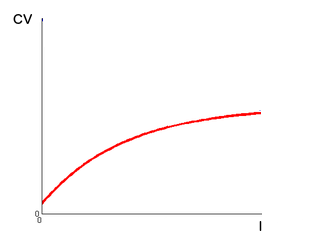
\includegraphics[width=0.7 \textwidth]{images/learning_curve1}
\end{frame}
}

\begin{frame}{Критерий непротиворечивости моделей}  
  \alert{Идея}: Если модель верна, то алгоритмы, настроенные по разным частям данных, не должны противоречить друг другу.\\
\end{frame}

\section{Аналитический подход}

\begin{frame}{Как использовать аналитические оценки}  
  \begin{enumerate}
    \item Получить верхнюю оценку вероятности переобучения\\
      $$P[E_{out} - E_{in} > \varepsilon] \leq \eta(\varepsilon)$$
    \item Тогда с вероятностью не менее $1-\eta$ справедливо\\
      $$E_{out} < E_{in} + \varepsilon(\eta)$$
    \item Будем оптимизивать \\
      $$E_{in} + \varepsilon(\eta) \rightarrow \min\limits_{\mu}$$
  \end{enumerate}
\end{frame}

\begin{frame}{Регуляризация}
  Регуляризатор $\varepsilon$ — аддитивная добавка к внутреннему критерию, штраф за сложность модели A.
\end{frame}

\begin{frame}{Неравенство Бернштейна-Хёфдинга}
  \begin{minipage}[t]{0.5\linewidth}
    $$P[\vert a - b \vert > \varepsilon ] \leq 2 e^{-2 \varepsilon^2 l} $$\\
  \end{minipage}%
  \begin{minipage}{0.45\textwidth}
    \begin{center}
      \begin{figure}
        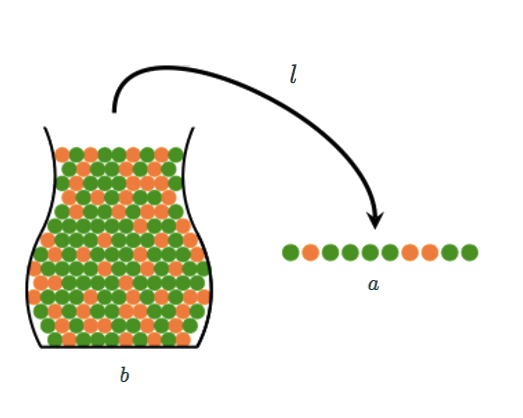
\includegraphics[width=\textwidth, keepaspectratio]{images/bin}    
      \end{figure}
    \end{center}

  \end{minipage}%
    \bigbreak
    $a$ -- доля оранжевых шаров в выборке размера $l$\\
    $b$ -- истинная доля оранжевых шаров 
  
\end{frame}

\section{Какое отношение это имеет к нашим моделям?}

\begin{frame}
  Каждый шар это объект $x$ из пространства $X$.\\
  Неизвестная целевая функция $f$.\\
  \bigbreak
  Зелёный шар -- модель $h$ верна ($h(x) = f(x)$)\\  
  Оранжевый шар -- модель $h$ не верна ($h(x) \neq f(x)$)\\  
  \bigbreak
  По выборке $X^l$ можем оценить долю объектов, на которых модель ошибается.
\end{frame}

\begin{frame}{$E_{in}$ и $E_{out}$}
  $E_{in}(h) = a$ - доля объектов в выборке $X^l$, на которых $h$ ошибается\\
  $E_{out}(h) = b$ - доля объектов во всём множестве $X$, на которых $h$ ошибается\\
  \bigbreak
  $$P[\vert E_{in}(h) - E_{out}(h) \vert > \varepsilon ] \leq 2 e^{-2 \varepsilon^2 l} $$\\
  \bigbreak
  Неравенство выполняется для каждой модели.
\end{frame}

\begin{frame}{Важная деталь}
  \centering
  Какова вероятность, что модель $a \in A$, наилучшим образом приближающая $f$ по выборке, наилучшим образом приближает $f$ на всём множестве?
\end{frame}

\begin{frame}{Простая аналогия}
  \centering
  С какой вероятностью монета, подброшенная 10 раз, выпадет одной и той же стороной все 10 раз?
  \pause
  \bigbreak
  \textcolor{blue}{$0.001$}
\end{frame}

\begin{frame}{Простая аналогия}
  \centering
  С какой вероятностью одна из 1000 монет, каждая из которых подброшена 10 раз, выпадет одной и той же стороной все 10 раз?
  \pause
  \bigbreak
  \textcolor{blue}{$0.63$}
\end{frame}

\begin{frame} {К нашей задаче}
  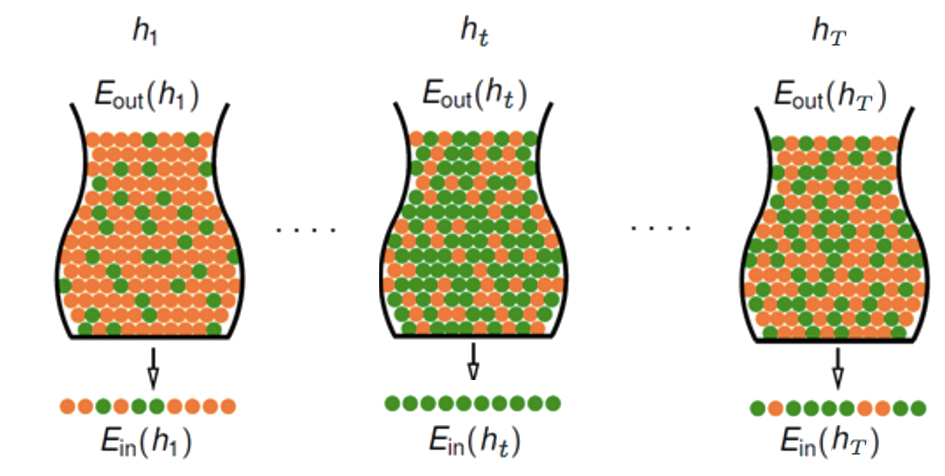
\includegraphics[width=\textwidth, keepaspectratio]{images/bins}
  
  На $h_t$ модели наблюдаем переобучение.
\end{frame}

\begin{frame} {Решение}
  \begin{align*}
    P[\vert E_{in}(a) - E_{out}(a) \vert > \varepsilon ] &\leq \sum\limits_{t=1}^T P[\vert E_{in}(h) - E_{out}(h) \vert > \varepsilon ] \\
    & \leq 2\textcolor{orange}{T} e^{-2 \varepsilon^2 l} 
  \end{align*}
\end{frame}

%{\foot{loss function}
%\begin{frame}{Функция потерь}
%  Задача классификации:\\
%  $\mathcal{L}(h, x_i) = [h(x_i) \neq y_i]$ -- индикатор ошибки\\
%  \bigbreak
%  Задача регрессии:\\
%  $\mathcal{L}(h, x_i) = \vert h(x_i) - y_i \vert$ -- абсолютное значение ошибки\\
%  $\mathcal{L}(h, x_i) = (h(x_i) - y_i)^2$ -- квадратичная ошибка\\
%\end{frame}
%}

%{\foot{функционал средних потерь, Empirical Risk}
%\begin{frame}{Функционал качества}
%  Функционал качества гипотезы $h$ на выборке $X^l$:\\
%  $$E_{in}(h, X^l) = \frac{1}{l} \sum\limits_{i=1}^l \mathcal{L}(h, x_i)$$\\
%  Минимизация эмпирического риска:\\
%  $$\arg\min\limits_{h} E_{in}(h, X^l)$$
%\end{frame}
%}

%\begin{frame}{Полная и поточечная ошибка}  
%  $$E_{in}(h, X^l) = \frac{1}{l} \sum\limits_{i=1}^l \mathcal{L}(h, x_i)$$\\
%  \bigbreak
%  $$E_{out} = \mathbb{E}_x \mathcal{L}(h, x) $$
%\end{frame}

%\begin{frame}{Шум в наблюдениях}  
%  Что делать, если два абсолютно одинаковых объекта выборки (с точки зрения параметров) имеют разные значения $y$?
%\end{frame}
%
%\begin{frame}{Шум в наблюдениях}  
%  Будем использовать целевое распределение вместо целевой функции:\\
%  $$p(y|x)$$\\
%  Пара $(x, y)$ генерируется распределением:\\
%  $$P_x p(y|x)$$\\
%  Целевая функция выглядит так:\\
%  $f(x) = \mathbb{E}(y|x)$ + шум $y - f(x)$
%\end{frame}

%\begin{frame}{Обучение в терминах вероятности}  
%  В идеале хотим достичь $E_{out}(a) = 0$\\
%  \bigbreak
%  Пытаемся достичь $E_{in}(a) \approx E_{out}(a)$ и $E_{in}(a) = 0$
%  \bigbreak
%  \pause
%  Два вопроса:\\
%  \begin{enumerate}
%    \item Можно ли судить о $E_{out}$ по $E_{in}$?
%    \item Как уменьшить $E_{in}$?
%  \end{enumerate}
%\end{frame}
%
%\begin{frame}{Сложность модели}  
%  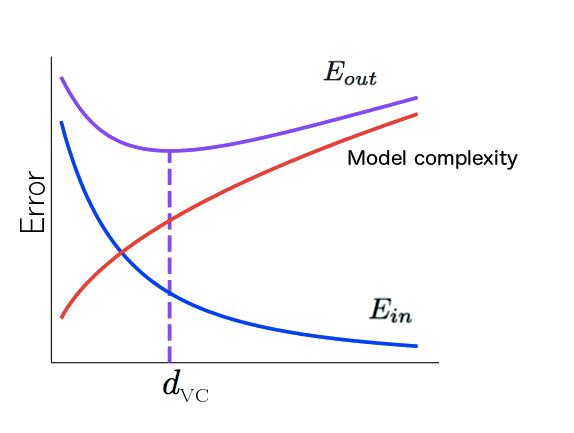
\includegraphics[ width=\textwidth, keepaspectratio]{images/vc}
%\end{frame}

\section{Какое количество моделей в нашем пространстве $A$?}

\begin{frame}{Близость моделей} 
  \centering 
  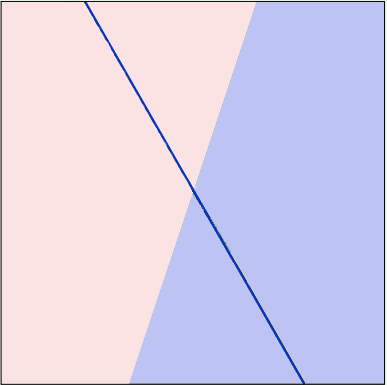
\includegraphics[ width=0.6 \textwidth, keepaspectratio]{images/hypothesis1}
\end{frame}

\begin{frame}{Близость моделей}  
  \centering
  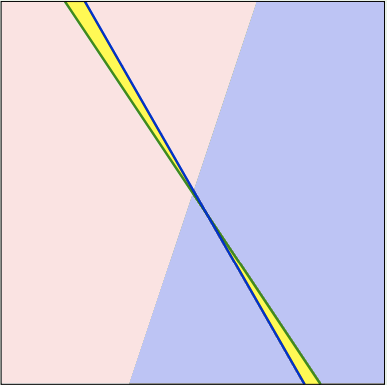
\includegraphics[ width=0.6 \textwidth, keepaspectratio]{images/hypothesis}
\end{frame}

\begin{frame}{Близость моделей}  
  $\bigtriangleup E_{out} = $ площадь жёлтой области\\
  \bigbreak
  $\bigtriangleup E_{in} = $ изменение меток объектов жёлтой области в выборке\\
  \bigbreak
  $\vert E_{in}(h_1) - E_{out}(h1) \vert \approx \vert E_{in}(h_2) - E_{out}(h2) \vert$  
\end{frame}

\begin{frame}{Вопрос}  
  \begin{minipage}[t]{0.5\linewidth}
    \begin{flushleft}
    Обучающая выборка $x_1, \dots, x_l$ и набор бинарных значений меток $y_1,\dots,y_l$.\\
    \end{flushleft}
  \end{minipage}%
  \begin{minipage}{0.5\linewidth}
      \centering
        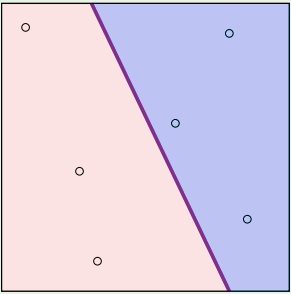
\includegraphics[width=0.8 \textwidth, keepaspectratio]{images/dich}    
  \end{minipage}%  
  \centering  
  \bigbreak
  Сколько вариантов $y_1,\dots, y_l$? 
\end{frame}

{\foot{коэффициент разнообразия}
\begin{frame}{Дихотомии}  
  $$P(\vert E_{in}(a) - E_{out}(a) \vert > \varepsilon) \leq 2 T e^{-2\varepsilon^2l}$$  \\
  \bigbreak
  Наш набор моделей $A$ может породить $\vert A(x_1,\dots, x_l) \vert$ дихотомий.\\
  $$\vert A(x_1,\dots, x_l) \vert \leq 2^l$$\\
  При этом сам набор моделей может быть бесконечным.
\end{frame}
}

\begin{frame}{Функция роста $m_{A}(l)$}  
  \centering
  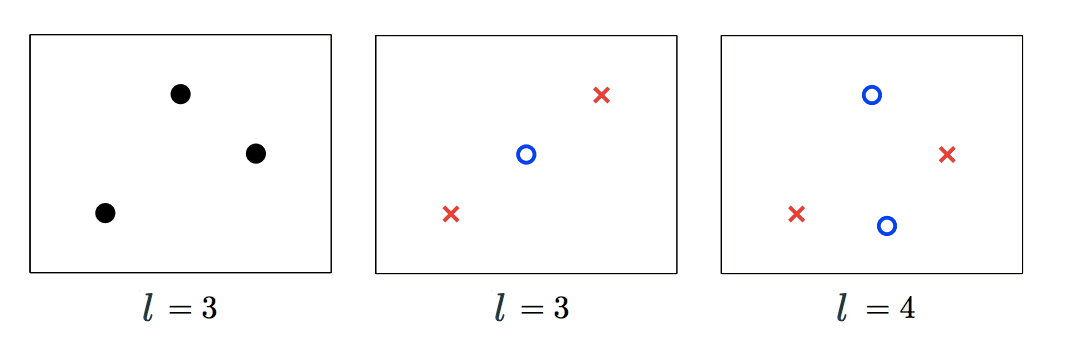
\includegraphics[width=\textwidth, keepaspectratio]{images/growth}
  $$m_{A}(l) = \max\limits_{x_1,\dots,x_l} \vert A(x_1,\dots, x_l) \vert \leq 2^l$$\\
\end{frame}

%\begin{frame} {Функция роста $m_{A(l)}$}
%  Модели:\\  
%  \begin{enumerate}
%    \item Луч на множестве точек: $m_{A}(l) = l+1 $
%    \item Интервал на множестве точек: $m_{A}(l) = C_{l+1}^2 + 1$
%    \item Выпуклое множество на множестве точек: $m_{A}(l) = 2^l$ 
%  \end{enumerate}
%\end{frame}

{\foot{точка поломки, break point}
\begin{frame}{Точка разрыва}  
  Если для некоторого $k$ выполняется $m_{A}(k) < 2^k$, то $k$ называется точкой разрыва.
\end{frame}
}

\begin{frame}{Точка разрыва}  
  \centering
  Наличие точки разрыва означает наличие полиномиального ограничения на функцию роста $m_{A}(l)$
\end{frame}

\begin{frame}{Пример}  
  \centering
  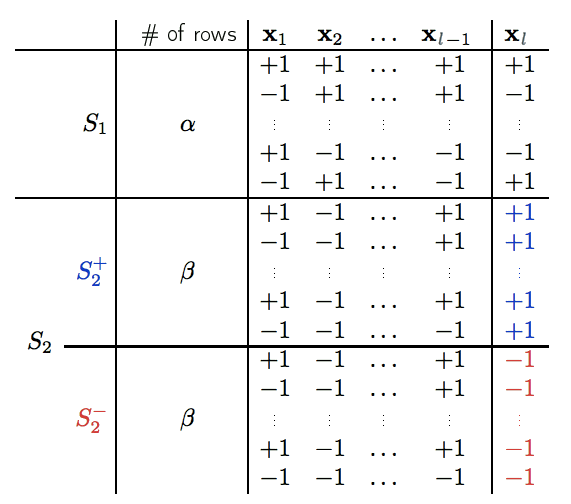
\includegraphics[width=\textwidth, height=0.8 \textheight, keepaspectratio]{images/breakpoint}\\
  Разделим на 2 ситуации относительно $x_l$: \\либо есть только один вариант (+1 или -1), либо оба (+1 и -1)
\end{frame}

\begin{frame}{Число дихотомий}  
  $B(l, k)$ -- максимальное число дихотомий для выборки размера $l$ при наличии точки разрыва $k$.\\
  \bigbreak
  \begin{itemize}
    \item $B(l, k) = \alpha  + 2\beta$
    \item $\alpha + \beta \leq B(l-1, k)$\\
    \item $\beta \leq B(l-1, k-1)$ 
  \end{itemize}
  $\implies B(l, k) \leq B(l-1, k) + B(l-1, k-1)$
\end{frame}

\begin{frame}{Оценка $\alpha + \beta$}  
  \centering
  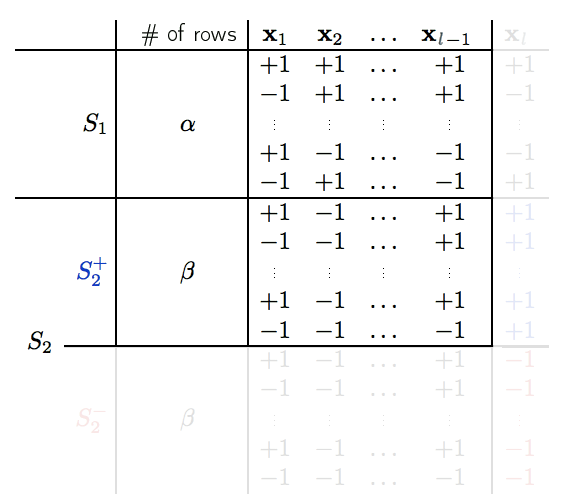
\includegraphics[width=\textwidth, height=0.8 \textheight, keepaspectratio]{images/breakpoint1}
\end{frame}

\begin{frame}{Оценка $\beta$}  
  \centering
  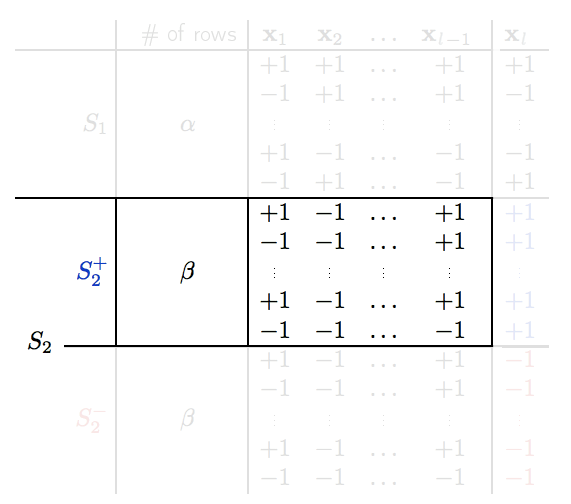
\includegraphics[width=\textwidth, height=0.8 \textheight, keepaspectratio]{images/breakpoint2}
\end{frame}

\begin{frame}{Число дихотомий}  
  $$B(l, k) \leq \sum\limits_{i=0}^{k-1} C_l^i$$\\
  Доказывается по индукции:\\
    \bigbreak
  $B(l, 1) = 1 $, \space $B(1, k) = 2 $\\
  \bigbreak
  Индукционный шаг:
  $\sum\limits_{i=0}^{k-1} C_l^i = \sum\limits_{i=0}^{k-1} C_{l-1}^i + \sum\limits_{i=0}^{k-2} C_l^i$
\end{frame}

\begin{frame}{Полиномиальное ограничение}  
  $$m_{A}(l) \leq B(l, k) \leq \sum\limits_{i=0}^{k-1} C_l^i \leq l^{k-1}$$\\
\end{frame}

\begin{frame}{Финальное неравенство}  
  $$P(E_{in}(a) - E_{out}(a) > \varepsilon) \leq 2 l^{k-1} e^{-2 \varepsilon^2 l}$$\\
\end{frame}

\begin{frame}{Неравенство Вапника-Червоненкиса}  
  $$P(E_{in}(a) - E_{out}(a) > \varepsilon) \leq 4 m_{A}(2l) e^{-\frac{1}{8}\varepsilon^2l}$$\\
  \bigbreak
\end{frame}

%\begin{frame}{Сложность модели}  
%  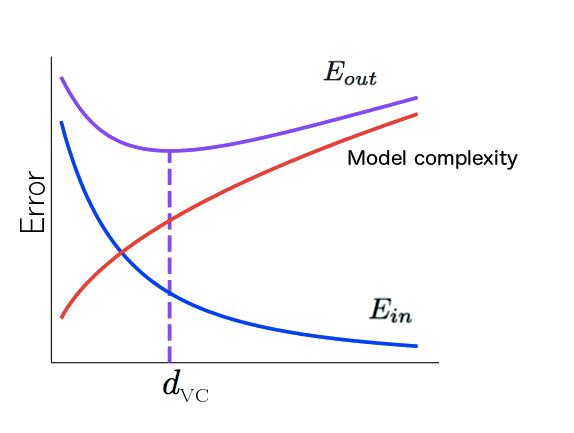
\includegraphics[ width=\textwidth, keepaspectratio]{images/vc}
%\end{frame}

{\foot{$L_2$-регуляризация, ридж, weight-decay}
\begin{frame}\frametitle{Пример регуляризации в градиентном спуске}
	Функционал с регуляризацией:\\
	$Q_{\tau} = Q + \frac{\tau}{2}\Vert \mathbf{w} \Vert^2 \rightarrow \min\limits_{\mathbf{w}}$\\
	\bigbreak
	Градиент:\\
	$\bigtriangledown Q_{\tau} = \bigtriangledown Q + \tau \mathbf{w}$\\
	\bigbreak
	Градиентный шаг:\\
	$\mathbf{w} = \mathbf{w}(1-\alpha \tau) - \alpha \bigtriangledown Q(\mathbf{w})$\\
\end{frame}
}

\begin{frame}[standout]
  Вопросы?
\end{frame}

\appendix

\begin{frame}\frametitle{Что почитать по этой лекции}
  \begin{itemize}
    \item \href{http://work.caltech.edu/telecourse.html}{Professor Yaser Abu-Mostafa MOOC}
    \item Tom Mitchell "Machine Learning" Chapter 4
    \item  Hastie, T., Tibshirani R. "The Elements of Statistical Learning" Chapter 7.9 
  \end{itemize}
\end{frame}

\begin{frame}\frametitle{На следующей лекции}
	\begin{itemize}
    	\item[--] Многослойная нейронная сеть
    	\item[--] Нелинейное преобразование
    	\item[--] Быстрое вычисление градиента
    	\item[--] Алгоритм обратного распространения ошибки
    	\item[--] Оптимизация структуры сети
    	\item[--] Сверточные нейросети   	    	
	\end{itemize}
\end{frame}
\end{document}

\end{document}